% vim: foldmarker=\Section,%EndSection
% vim: syntax=off

\documentclass [11pt] {jsarticle}

\newcommand\Section[1]{\newpage \section {#1}}

\usepackage [hmargin={2.0cm,2.0cm},vmargin={2.0cm,3.0cm}] {geometry}
\usepackage [dvipdfm] {graphicx}
\usepackage [dvipdfm,table]{xcolor}
\usepackage {amsmath,floatflt,url,alltt}

\definecolor{bgcolor}{gray}{0.85}

\pagestyle {empty}

\newcommand\raisedrule[2][0em]{\leaders\hbox{\rule[#1]{1pt}{#2}}\hfill}
\newcommand\HFill{\hspace {1zw}\raisedrule[1ex]{.5pt}\hspace {1zw}}

\newcommand\var[1]{\textrm {\textit {#1}}}
\newcommand\rsv[1]{\textrm {\textbf {#1}}}
\newcommand\mth[1]{\textrm {\textsf {#1}}}
\newcommand\cls[1]{\textrm {\textsf {#1}}}

\renewcommand\abstractname {概要/Abstract}
\title {ビジュアルプログラミングについての一考察\\ A Thought on Visual Programming}
\author {脇田 建/Ken Wakita\\
東京工業大学大学院 数理・計算科学専攻\\[1ex]
Department of Mathematical and Computing Sciences, \\
Tokyo Institute of Technology}
\date {}

%EndSection

\begin {document}

\maketitle
\thispagestyle {empty}

\begin {abstract}
今年の夏学期に初年次情報教育で始めてMIT Scratchを用いてプログラミング実習を行った.ビジュアル言語の効果は計り知れなかった.伝統的なプログラミング教育で多くの優秀な学生の理解を阻んだ内容を,専門教育を受けていない学生たちはいとも軽々と乗り越えていった.本稿では,ビジュアルプログラミング言語と従来のプログラミング言語の本質的な差を\emph {構造化}と見定め,ビジュアル言語の利点を説き,その将来性について論じる.\footnote {ページ数の制限から本稿に書ききれなかった内容も多々あります.今後,内容をさらに充実させたものを随時公表していこうと思っております.本稿の内容にご興味をいただきましたら,このURL (\url {feed:https://github.com/wakita/visual_programming_paper/commits/master.atom}) をご購読下さい.}\bigskip

During a programming course that the author gave to freshmen for this summer semester, he was severely shocked to see them happily learning with MIT Scratch, who often find difficulty in learning traditional text-based programming languages.  Based on the insight that the essence of visual programming as \emph {structured-ness}, the article demonstrates advantages of visual programming and its future potential.
\end {abstract}

\Section {私家版ビジュアルプログラミング
\HFill 構造化と見極めたり}

\begin {figure}
\centerline {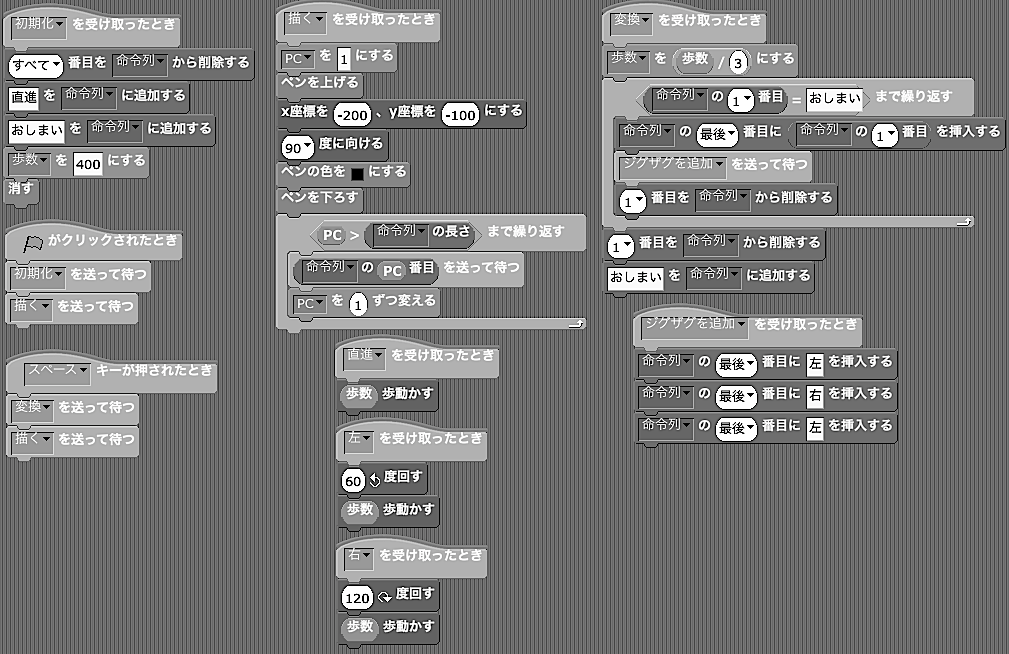
\includegraphics [width=.95\linewidth] {figs/scratch-program.png}}
\caption {MIT Scratchで記述したKoch曲線を描くプログラムの記述例}
\label {fig: an example of Scratch program}
\end {figure}

ビジュアルプログラミング言語とは,従来のテキストで記述するプログラミング言語に対して,そうではないもの,そしてプログラミングにおける諸概念を図示したものとして理解されているように思う.本稿を執筆するにあたって,この漠然とした考え方よりはかなり狭い意味における\emph {私家版ビジュアルプログラミング}を説明したい.

まず,既存のビジュアルプログラミング言語の代表としてMIT Media Lab. で開発された\emph {Scratch}\cite {esnick09Scratch:-Programming-for-All}\footnote {\url {http://scratch.mit.edu/}}を取り上げる(図\ref {fig: an example of Scratch program}参照).ScratchはLOGO\cite {Papert80Mindstorms:-children-computers}, Lego Mindstorm\footnote {\url {http://mindstorms.lego.com/}}, Scratch と MIT で 30年にわたる研究活動の最新の成果である.この言語はいくつかの意味でビジュアルである.

\begin {floatingfigure}[r]{.10\linewidth}

\includegraphics [height=7ex] {figs/scratch-sprite.png}
\end {floatingfigure}
第一に,Scratchを起動すると現れる猫の振る舞いを記述することがScratchにおけるプログラミングの基本である.プログラムの動作の結果は猫の動作として可視的にフィードバックされる意味においてプログラミングの効果がビジュアルである.

\begin {floatingfigure}[r]{.16\linewidth}

\includegraphics [height=7ex] {figs/scratch-block.png}
\end {floatingfigure}
次に,Scratch におけるプログラムは,ブロックを組み合わせ,パラメターを指定することによって記述される.プログラミング言語の構文要素を文字を連ねて記述するかわりに,構文構造に対応したブロックを\emph {直接操作} (\emph {direct manipulation})して組み合わせる点,すなわちプログラムを構築する作業がユーザインタフェイスを通して行われる点でビジュアルである.

最後に,Scratchのプログラムの状態は基本的には,猫の位置と速度と向きといった物理状態の他,コスチュームと呼ばれる見た目の様子などのわずかな状態量を基本としているが,より複雑な振る舞いを記述する目的で変数やリストも利用できる.これらに代入された値を猫の振る舞いから推し量ることは困難である.そのため,Scratchは必要に応じて変数やリストをモニターする機能があり,これを簡易ビジュアルデバッガと見ることもできる.この意味でもビジュアルといえる.
\begin {floatingfigure}[r]{.32\linewidth}

\includegraphics [height=7ex] {figs/scratch-state.png}
\end {floatingfigure}

本稿が対象とするビジュアルプログラミング言語は,第一,あるいは第三の可視性よりもむしろ,第二の構文要素(抽象構文木の要素)が直接操作できる点を重視する.以下では,この構文要素だけでなく,プログラム実行中のデータを含めた\emph {プログラミングにおける諸概念を直接操作できることをビジュアルプログラミングの本質}とした上で,このことがプログラミング作業,プログラミング言語の設計と実装とどのように関わるのかを論ずる.

従来のプログラミング言語処理系はテキストで記述されたプログラムを入力とし,その内容に応じて処理を行ってきた.プログラムの処理においては,普通はプログラムをトークン列に分解してから,構文解析によって抽象構文木を構成する.抽象構文木はプログラムに記載された内容のうち,プログラムの意味を司るすべてを網羅したデータ構造である.この意味で,プログラミング言語においては抽象構文木こそがプログラムの意味を表していると考えるべきであろう.一方,プログラムは抽象構文木の内容をテキストで表現するための形式で記述されている.プログラムのテキスト表現には,構文理論上の曖昧性を排除しつつ,抽象構文木を構成するために十分な情報を含むことが求められる.したがって\emph {具象構文}と呼ばれるプログラムの字面上の文法は抽象構文に比べると格段に複雑である.

例えば,整数を含む配列の内容を1ずつ増加するJavaのプログラムについて考えてみよう.以下のコードのなかでいくつの句読点の類いが用いられているだろうか.セミコロンが3箇所,括弧と波括弧が対をなし,あわせて7つの記号が用いられている.これらの記号の目的は,以下のコードを正確に構文解析することにある.実際,Javaの抽象構文木にセミコロン,括弧,波括弧はない.\bigskip

\begin {tabular}{cc}
\begin {minipage}[b]{.48\linewidth}
\begin{alltt}
\rsv{for} (\rsv{int} \var{i} = 0; \var{i} < \var{v}.\mth{length}; \var{i}++) \{
    \var{v}[\var{i}]++;
\}

\end{alltt}
\end {minipage} &
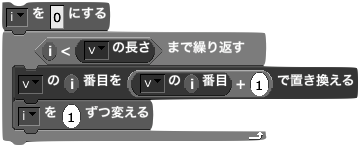
\includegraphics [width=.45\linewidth] {figs/scratch-scan-array.png}
\end {tabular}\bigskip

宮下らが超好意的解釈をする言語処理系\cite{Nakahashi10HMMMML2}の設計にあたって行った調査内容から見えてくるのは,プログラムの実行にとって非本質的な言語要素が初級プログラマを苦しめている事実である.

逆に,抽象構文木が直接扱えるということは,従来のプログラミング言語から構文解析のみのために必要とされ,構文解析以後は不要となる瑣末なものを一切除去できることを意味している.これにより,これまで我々を悩ませてきた文法上の間違いは一掃されることであろう.

抽象構文木を直接編集する限り,具象構文は不要となる.この意味でビジュアルプログラミング言語は具象構文を持たないプログラミング言語と言ってよい.すでに述べたように,句読点の有無などは具象構文の構文解析にとってのみ必要とされる.したがって,LISPに対する括弧の多寡,行末のセミコロンの省略への対応の有無などといったことはビジュアルプログラミング言語にとっては無意味な議論である.

%EndSection

\Section {ビジュアルプログラミング言語が変える言語実装法}

コンパイラの標準的な教科書を開いてみよう.たとえば,Ahoらにコンパイラの名著の場合\cite {Aho06Compilers:-Principles-techniques},全12章のうち,第2章から第4章までが字句解析と構文解析などのコンパイラ前処理部に割かれており,さらに付録全体(Appendix A: Complete Front End)も前処理部の事例となっている.

すでに述べたように,前処理部の目的はテキスト形式で表現されたプログラムを構文解析して抽象構文木を作成することにある.もし,プログラムが抽象構文木を直接編集しながら構成されていたとしたら,テキスト形式のプログラムを構文解析する必要はなくなる.ビジュアルプログラミングが普及すれば,プログラミング言語の開発者は最適化やコード生成のようなプログラミング言語のより本質的な仕事に注力できるだろう.

それでも注意深い読者は,GUIを通して作成されたプログラムをどのように保存すればよいのか,もしテキスト形式で保存するのであればもとの黙阿弥ではないかと心配になるかもしれない.プログラムの保存方法については,抽象構文木を編集していたときのメモリー状態をそのまま記録すればよい.メモリダンプでも,データの直列化(serialize)でも構わないだろうが,抽象構文木の構造を保存した形式で保存することが重要である.

ビジュアルプログラミング言語のエディタに求められる中心的な機能は,抽象構文木の編集である.基本的には,複数の子ノードからなる森を親ノードでまとめるボトムアップな編集と,親ノードの穴を漸次埋めていくトップダウンな編集に加えて,既存の子ノードを別の木で置き換える操作が求められるであろう.\cite {sasaki10GUI-component-visual}

\begin {floatingfigure}[r]{.30\linewidth}
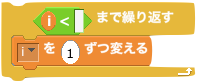
\includegraphics [width=.25\linewidth] {figs/scratch-sentential.png}
\end {floatingfigure}
いずれの編集作業においても,編集中のプログラムが未完成であることを考えると,実際に編集している時点では抽象構文木も未完成である.このような未完成の抽象構文木は,\emph {文形式} (\emph {sentential form})として形式化することができる.文脈自由文法で表された抽象構文$G = (N, T, P, S)$の文形式とは,非終端記号$X$から導出される文法記号の列$\alpha$のことである.たとえば,右図は\rsv {while}文に相当する非終端記号から以下のように導出された文形式と考えることができる.


\begin {quote}
\rsv {while} □ □ → 
\rsv {while} □ \fbox {\rsv {assign} □ □} → \\ \smallskip
\rsv {while} \fbox {□ $<$ □} \fbox {\rsv {assign} □ □} → 
\rsv {while} \fbox {□ $<$ □} \fbox {\rsv {assign} \fbox {\var {i}} □} → \\ \smallskip
\rsv {while} \fbox {\fbox {\var {i}} $<$ □} \fbox {\rsv {assign} \fbox {\var {i}} □} →
\rsv {while} \fbox {\fbox {\var {i}} $<$ □} \fbox {\rsv {assign} \fbox {\var {i}} \fbox {\fbox {\var {i}} + \fbox {1}}}
\end {quote}

そして,図中の穴に変数$n$を表すブロックを埋め込む操作は,最後の文形式のなかの穴(□)からこの変数を表す終端記号$n$を導出する操作に過ぎない.MIT Scratchではブロックの穴に別のブロック群をドラッグ&ドロップ操作で埋めるときに,この組み合わせが抽象構文において妥当な組み合わせか否かを検査する.この検査は,実は穴に対応する非終端記号からブロック群のもととなっている非終端記号を直接的に導出できるか否かを判定しているにすぎないため容易に実装することができる.

たとえば,上図の穴に変数を表すブロックをドロップすることは許されるが,文を表すブロックをドロップをドロップすることは許されない.このことは穴に対応する非終端記号が式であるため,「式 → 変数」という導出規則は存在しても,「式 → 文」という導出規則がないことから判定できる.

%EndSection

\Section {見えているものは正しい
\HFill 可視性}

\centerline {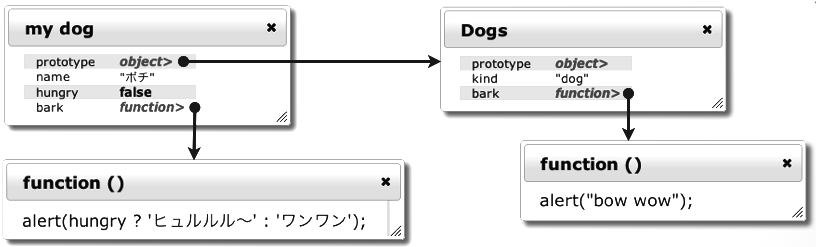
\includegraphics [width=.8\linewidth] {figs/core-pochi.png}}

ビジュアルプログラミングにおける\emph {ビジュアル}とはプログラミングに関わる諸概念が可視化されることを意味する.すでにプログラムの構造を可視化し,直接操作することの重要性について論じたが,ここではプログラムが扱う\emph {データの可視化とその直接操作}について論じたい.プログラムが扱う任意のデータを表示し,操作する機能はプログラムのデバッグに欠かすことができない.そこでは,単純なヴィジュアリゼイションと異なり,コンピュータ内のデータの内容を忠実に表示するだけでなく,表示されたものを直接的に操作してデータの内容を更新できることが求められる.すなわち,編集対象となっているコンピュータ内のデータとその画面表示との間の一貫性と保つことが重要である.

上図は犬を仮想化したオブジェクトの画面表示である.一般的な犬の概念を表す\cls {Dogs} オブジェクトを元に我が家の愛犬ポチを表す\cls {my dog}オブジェクトが構成されている.この例では一般的な犬は``Bow wow''と吠えるが,ポチは普段は``ワンワン''と吠え,空腹時は``ヒュルルルル〜''と飢餓を訴えることとしている.ポチの空腹感を表すために\cls {my dog}は\mth {hungry}フィールドを用意している.

この画面の\cls {my dog}の\mth {hungry}欄を修正して``\texttt {true}''と書き換えたならば,その瞬間にコンピュータ内部にあるポチに対応したオブジェクトの\mth {hungry}フィールドも\rsv {true}に更新され,したがってその状態で\mth {bark}メソッドが呼ばれたなら,ポチは``ヒュルルルル〜''と鳴くべきである.

また一方,プログラム実行の最中に ``\var {my dog}.\mth {hungry} ← \rsv {false}'' が実行され,ポチに対応したオブジェクトの\mth {hungry}の値が\rsv {true}から\rsv {false}に更新されたなら,その瞬間にこのオブジェクトに対応した,上図の\cls {my dog}の\mth {hungry}欄の表示も``\texttt {false}''から``\texttt {true}''に変化すべきである.

さて,システム内に数百万個ものオブジェクトがあったとして,それらすべての変化を監視しつつ,変化を逐一,画面に反映させるとしたら大変な計算コストがかかってしまう.実際に,そのようなことは不可能ではないだろうか.

もちろん,システム内のすべてのオブジェクトの変化を画面に実時間で反映させることは不可能である.しかしながら,人間が視認可能な変化に限れば,それは十分に可能である.如何にシステム内に存在するオブジェクトが多かったとしても,画面に表示できるデータの最大数は,画面の大きさと人間の目の解像度に依存した可視的な不動産の面積に制約され,さほど多くはない.どんなに多くても高々数千個といったところであろう.画面に表示されているフィールドに限ってObserverを設定すれば,多くの用途において十分に良好な反応性を実装できるであろう.ごく稀な例として,これらのフィールドが満遍なく,集中的に変化する場合には,仮に十分に高速に表示できたとしても,変化の速さは人間の認知の限界を越えてしまい意味がない.このような場合は情報の抽象化などの対応を検討すべきである.

% objects vs. visuals: causal relationship

%EndSection

\Section {百聞は一見にしかず
\HFill マルチメディア,国際化,複数ビュー}

ビジュアルプログラミングのもうひとつの利点は,プログラムがGUIを得ることによって,従来,テキストでの表現が困難だったものをプログラムに含めることができる点である.すなわち,テキストでは表現しにくい,マルチメディアコンテンツとしてのプログラムが作成できるようになる.映像コンテンツを表示し連続再生するプログラムを記述するのに,映像コンテンツを直接プログラミングシステムで開き,アイコンとして表示した上で,適宜,再生方式を設定してから,それを参照した関数に再生機能をプログラムできればどんなに楽だろう.\bigskip

\bgroup
\rowcolors {1}{bgcolor}{lightgray}
\begin {tabular}{cc}
\begin {minipage}[b]{.66\linewidth}
\begin{alltt}\renewcommand\baselinestretch{.85}\normalsize
[\cls{QTMovie} \var{movie} =
  [[\cls{QTMovie}
      \mth{movieNamed}: @"sample.mov"
      \mth{error}: &\var{error}]
   \mth{retain}];
[\var{movie}
  \mth{setAttribute}:[\cls{NSNumber} \mth{numberWithBool}:\rsv{YES}]
  \mth{forKey}: \rsv{QTMovieLoopsAttribute}];
[\var{movieView} \mth{setMovie}: \var{movie}]
[\var{movie} \mth{play}]
\end{alltt}
\end {minipage}
&
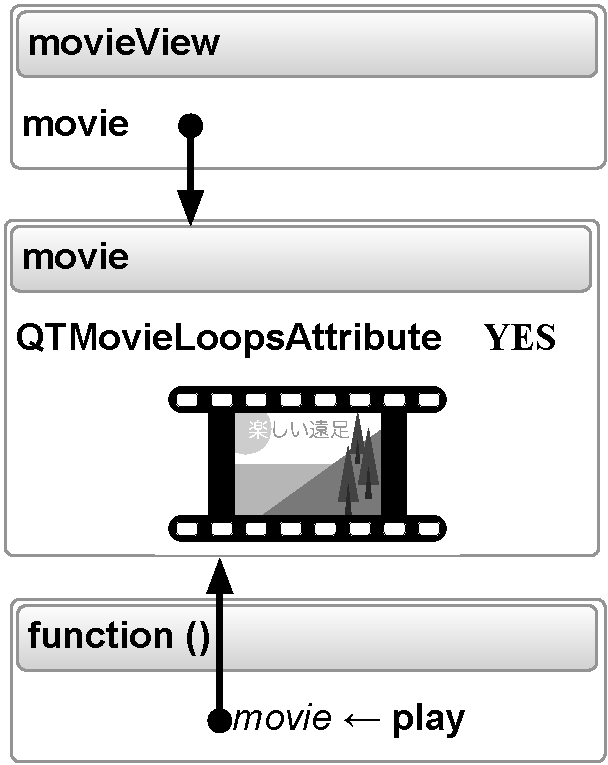
\includegraphics [width=.25\linewidth] {figs/movie-bg.pdf}
\end {tabular}
\egroup
\bigskip

\begin {floatingfigure}[r]{.30\linewidth}
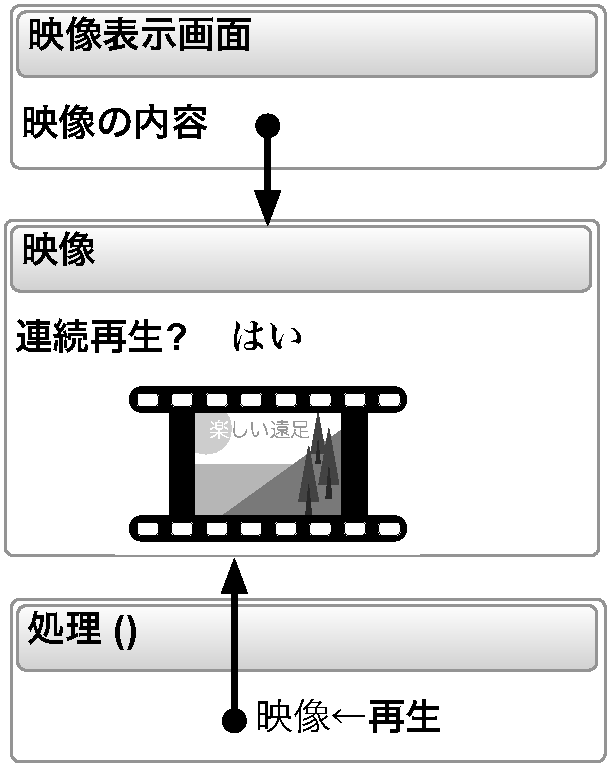
\includegraphics [width=.25\linewidth] {figs/movie-ja-bg.pdf}
\end {floatingfigure}
マルチメディアは複数のメディアを組み合わされてひとつのコンテンツを構成する技術である.このことはごく自然にコンテンツを構造化する技術を生んだ.コンテンツが構造化することによって,さまざまな利用シーンに対応して異なる方法でコンテンツを提示する技術も発展した.そのひとつの応用例が,ソフトウェアの多言語化である.本稿ではビジュアルプログラミングの本質をプログラミングにおける諸概念の構造化としているが,このことはごく自然にプログラムの多言語化を可能にするだろう.これまでも独自の国語を基礎としたプログラミング言語や,アプリケーションの国際化の例はあった.ビジュアルプログラミングの世界では,右図のように同じプログラミング言語を国際化して,複数の自然言語を通して見せることができるようになる.

ビジュアルプログラミングが提供するもう一つ可能性は,同じ概念に対する複数のビューを提供できる点である.MVC (Model-View-Control) モデルはひとつのデータに対して複数の見せ方を提供できる考え方である.たとえば数値の配列を考えてみよう.この配列の内容を子細に調査したい場合には,その要素のデータを閲覧したいだろう.この配列をソートした直後であれば,要素を折れ線グラフにプロットして表示すれば正しく正準化されているか容易に確認できる.この数値データが日本の海岸線の緯度経度を列挙したものであれば,それを散布図に表示すれば,データのなかに誤りがないか容易に確認できる.同じデータに対して必要に応じて異なるビューを与えることは,アプリケーションのユーザにとって便利なだけでなく,プログラマにとっても都合がよいに違いない.

% multiple views

%EndSection

\Section {頭に入る複雑さ
\HFill 文芸的プログラミングという抽象化}

仮にビジュアルプログラミングされたプログラムが理解しやすく,そのためプログラミングの生産性が飛躍的に向上したとしても,大規模なプログラミングができなければあまり大きな意味をもたない.はたして,ビジュアルプログラミングで大規模なシステムを構築することはできるだろうか.残念ながら既存のビジュアルプログラミングで大規模なシステムを記述した例はなく,たとえばビジュアルプログラミングシステムを用いて記述されたビジュアルプログラミングシステムというものも存在しない.

ビジュアルプログラミングにおいてはプログラミングにおける諸概念を可視化部品として表現して画面上に配置する.ひとつの画面に配置可能な可視化部品の点数には自ずから限度があり,それ以上に複雑なものを構成することはできない.MIT Scratch は巨大な仮想画面を用意してそこに自由に配置することを許しているが,実際に二次元的な広がりを持った仮想画面を上下左右にスクロールして閲覧することは困難である.テキストエディタでのスクロールが成功しているのは,テキストで記述されたプログラムが原則として上下方向の一次元的空間に記述されているためである.

このため,大規模なビジュアルプログラミングをするためにはソフトウェアを注意深くモジュール化し,画面の限られた空間に配置することが求められる.はたして,そのようなことは可能だろうか.以下では,安定性についての評価が高い中規模のソフトウェアの代表としてKnuth博士が実装した\TeX{}システムを例として見ていきたい.

以下の図は,\TeX のソースコード兼文書となる \texttt {tex.web}\footnote {\TeX{}システムのユーザならば,\texttt {"kpsewhich tex.web"}コマンドを実行すれば,このファイルを見つけられる.}のモジュールの大きさを棒グラフで表したものである.

\centerline {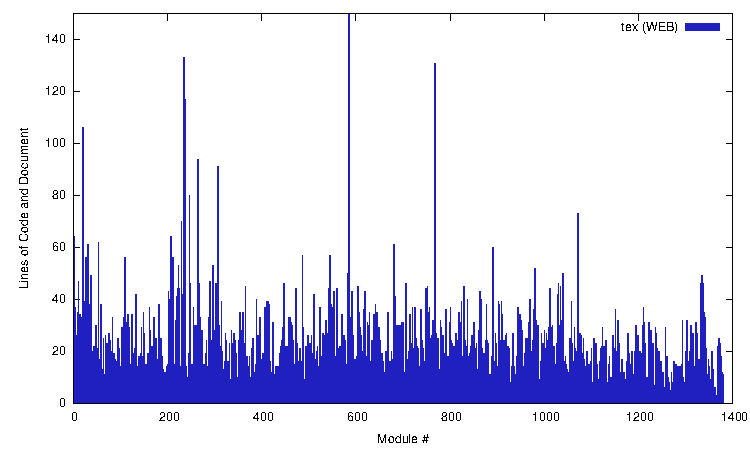
\includegraphics [width=.80\linewidth]{figs/web/tex-web.pdf}}

\TeX を構成する1379モジュールのうち,100行を越えるものは5つにすぎず,最大のものも237行のみである.しかも,ここでの行数はプログラムだけではなく,極めて念入りに叙述されたプログラムの説明を含めての分量であり,実際のプログラムの量はこれよりもかなり少ない.このことは\TeX に限ったことではなく,Knuth博士が書いたプログラムはすべてこの傾向にあることは次ページのデータが示している.

\newcommand\webfile[1]{\textbf {#1} &
  \includegraphics [height=3ex,width=.80\linewidth] {figs/web/#1-web.pdf}}

\begin {tabular}{ll}
  \webfile {gftodvi} \\
  \webfile {mf} \\
  \webfile {pltotf} \\
  \webfile {tangle} \\
  \webfile {tex} \\
  \webfile {vptovf} \\
  \webfile {weave}
\end {tabular}
\bigskip

1990年に発表された\TeX システム第3.0版は,その安定性についての定評が高い.実際,現在の最新版のバージョン番号(3.1415926)の小数点以下の桁数(=7)は,これまでに見つかった\TeX~3.0のバグの総数である.このように極めて安定したソフトウェアが構築された背景に\emph {文芸的プログラミング}\cite {Knuth92Literate-programming}\footnote {Literate Programming: \url {http://www.literateprogramming.com}}の大きな貢献を信じるのは私だけではないだろう.

\TeX システムのプログラムは文芸的プログラミングの実践の場であり,それを広く専門家の目に晒すことで世にその真価を問いかける場でもある.実際,\TeX システムの文書はそのまま書籍\cite {Knuth86TeX:-The-Program}として出版されたほどである.そのため,\TeX システムの記述にあたって,Knuthは\TeX システムのモジュール化と文書化には細心の注意を払ったものと想像される.

この事実から察することができるのは,かなりの規模のソフトウェアでも,優秀なソフトウェア開発者が注意深く設計・実装した場合には,比較的小さなモジュールの集りとして構成できるということである.このことは,さらに多くの検証を待つ必要がある.しかし,ビジュアルプログラミングにおいて,画面に収まる程度までモジュールの粒度を小さく保つことができる可能性を示唆していると考えてもよいだろう.むしろ,良質なソフトウェアを生産するためには,その程度までモジュールを小さく分割することこそが重要なのではないだろうか.

ところで,Knuthが始めた文芸的なプログラミングは単にプログラム中に大量のコメントを記述したものではない.文芸的なプログラミングでは,プログラムの一部に穴をあけ,別のモジュールを埋め込むようなことができる.たとえば,以下は筆者が試みに行った文芸的プログラミングの例\footnote {文芸的ウェブプログラミング: \url {http://ken-wakita.net/research/classes/cs1-2010/F1.pdf}}だが,ここで$\langle\text {と}\rangle$に囲われた箇所には,該当するモジュールが挿入される.通常のプログラミング言語には,クラス,関数,手続きといった抽象化機構は用意されているが,これらはプログラミング言語の文法の制約のなかで成立した機構である.文芸的プログラミングにおけるモジュールは,このような制約から脱皮することで,プログラムのより自由な抽象化を許し,従来は不可能であった抽象的な記述を可能としている.

\centerline {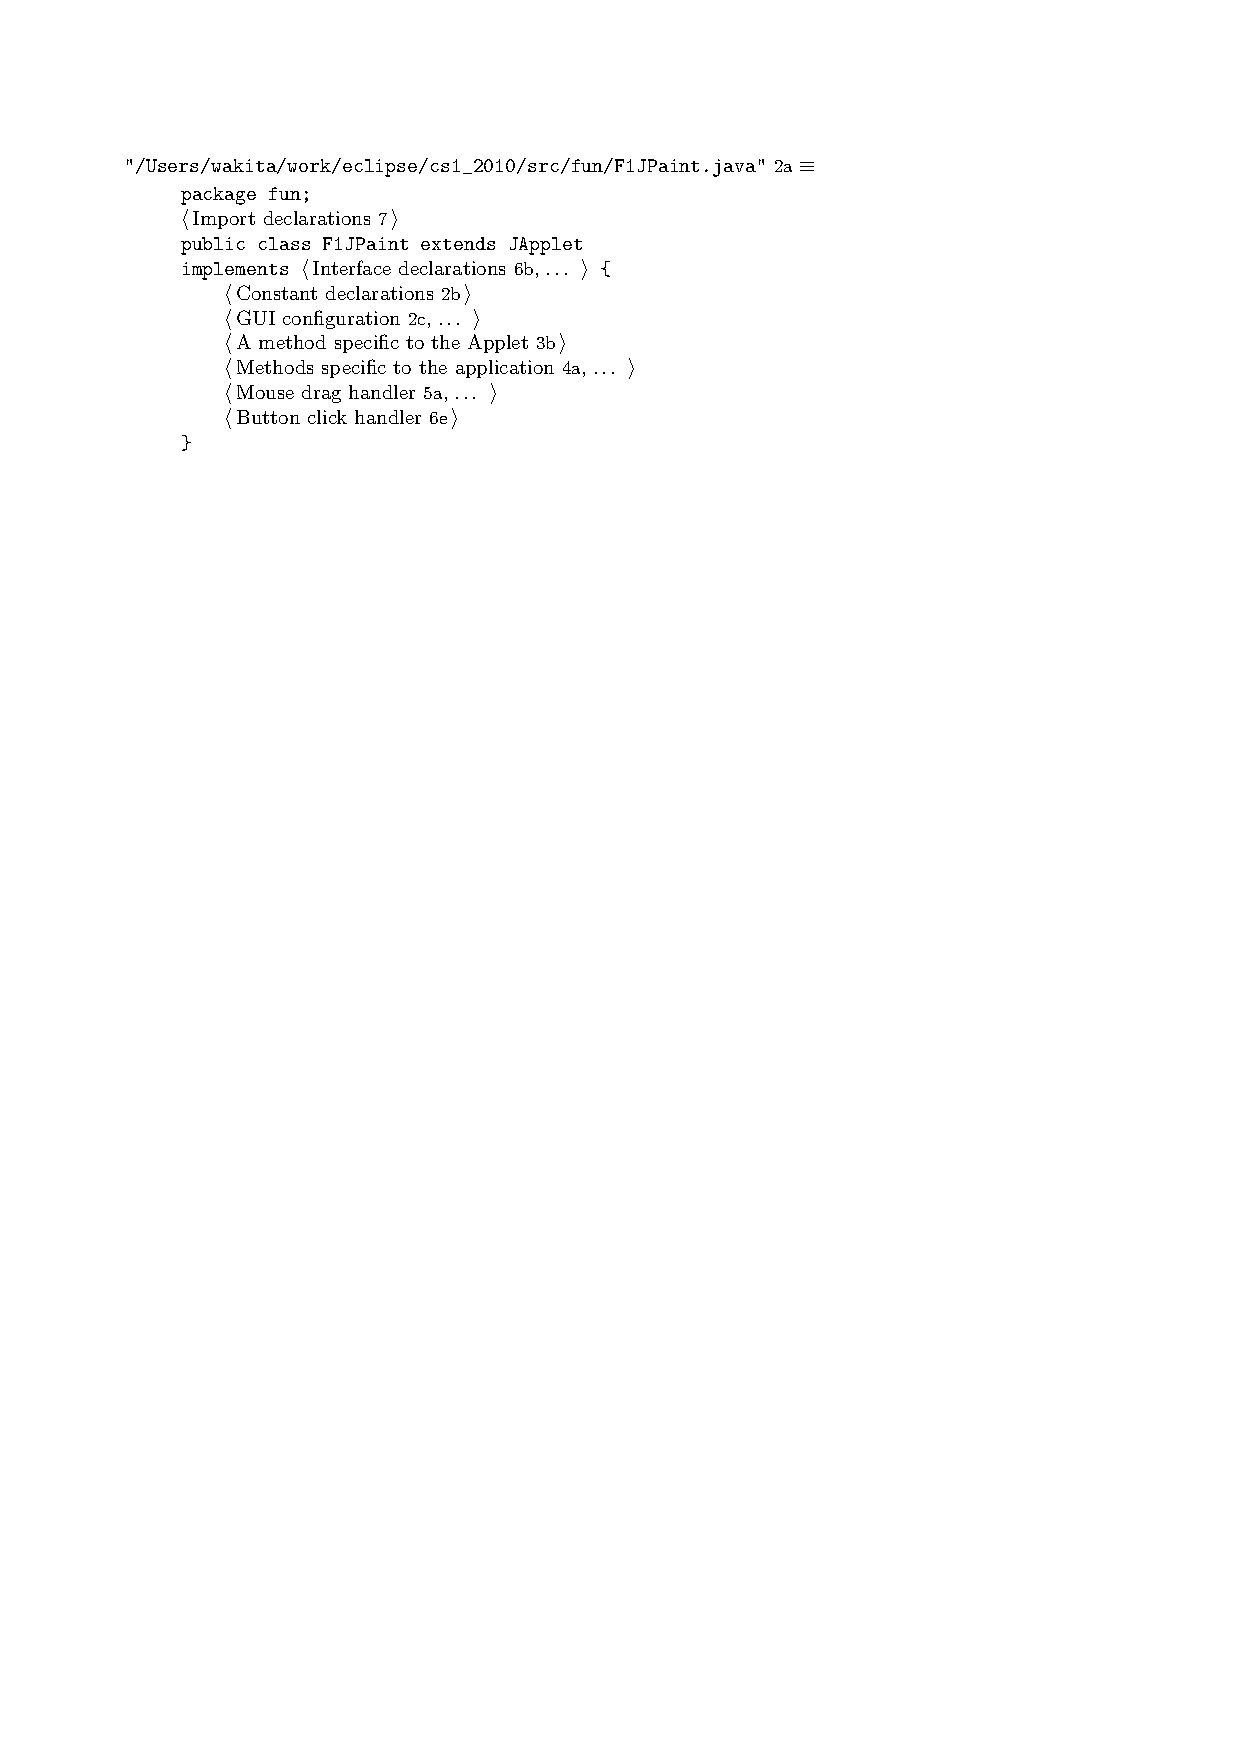
\includegraphics [scale=.85] {figs/F1JPaint.pdf}}

% abstraction (data, procedural, class-based)
% 理解に関する抽象化

%EndSection

\Section {ご質疑をいただきありがとうございました}

シンポジウムの場での質問やコメントに感謝しつつ.ご質問の内容にお答え申しあげます.

\begin {itemize}

\item オブジェクト=モノを強調すると抽象概念を表現できない人が生れる.
\HFill 伊知地宏さん\medskip

この発想はありませんでした.確かにそういう誤解を与える傾向があるかもしれません.今後,参考にして,誤解を与えないような工夫をしていきます.
\medskip

\item 再帰はどのように表現するのか?
\HFill 伊知地宏さん\medskip

再帰はプログラミングに欠かせないと思っています.今は(再帰を有する)ECMA Scriptの仕様を基礎にビジュアル言語を設計しています.再帰の記述については特別な工夫はありません.なお,児童向けのプログラミング言語として研究開発されてきたLOGO, Lego MindStorm, MIT Scratchの流れにおいて,元々LOGOにはあった再帰がいつのまにか欠落していました.これが教育心理学的な問題によるものか,そうではないのかは知らないのですが,その設計方針の変更については追っていきたいです.
\medskip

\item 100行のテキスト編集に比べて,そのGUIでの描画は大変ではないか?
\HFill 添田俊介さん\medskip

MIT Scratchの場合,制御構造ひとつを導入するだけで,制御構造の道具箱から拾ってくる操作をしなくてはならないため,熟練したプログラマがキーボードから簡単に入力することに比べてかなり面倒だと思います.ただ,この現状がビジュアルプログラミングの限界だと考えるのは間違いだと思います.今後,人間工学的に最適化することで,生産性をテキストエディタ以上に高めるようなプログラミング環境を開発すべきだと思っています.ただ,実のところコードの記述に関しては,テキストエディタとビジュアルエディタはあまり大きさ差はないのではないかという感触もあるのですが,それについては将来の研究を期待して下さい.
\medskip

\item 萩谷昌己さんのBoomborg\footnote {Boomborg-Keisan: \url {http://hagi.is.s.u-tokyo.ac.jp/boomborg/boomborg-keisan-j.html}}のような計算過程の可視化は考えているのか?
\HFill 伊知地宏さん\medskip

ビジュアルプログラミング環境として,プログラムが実行している最中に,そのプログラムのなかで操作されているデータやプログラム自身も修正することができるような環境を想定しています.プログラムの編集,実行,テストという開発における一連の流れを単一の環境で実現することが重要だと思います.そのなかで計算過程をもとにプログラムを構成することも考えております.
\medskip

\item Knuthのような天才でなくてもモジュール化できるのか?
\HFill 寺田実さん\medskip

今回はKnuthが書いたいくつかのソフトウェアのみを調べただけですので,十分な調査とは言えません.Scratchを使っていて感じたのですが,描画領域が限定されていることはむしろ無駄に長い記述を避け,簡潔な表現を求める動機づけとなります.本質的に複雑なプログラムを一定の面積にその詳細までを表現すること不可能ですので,そのためには一定の抽象化能力が求められます.すべての人が抽象化能力を持っているかどうかは不明ですが,少なくとも面積に関して制約を与えたビジュアルプログラミングがその訓練の場として利用できるでしょう.

\end {itemize}

%EndSection

\Section {おわりに}

この発表を通して訴えたかったことは,未来のプログラミング言語は従来のプログラミング言語とは大きく異なるということです.現在のプログラミング環境は20世紀に生み出されたものです.文字しか効率的に処理できなかった時代に比べて,ハードウェアは遥かに進歩しました.ITを巡る環境はマルチメディアに溢れかえっています.それなのに,どうしてプログラミング作業だけが旧態然としたテキストエディティングをしているのでしょう.

わたしには22世紀のプログラマがテキストエディタでプログラミングしている姿は想像できません.わたしはビジュアルプログラミングの未来を信じています.でも,それは間違っているかもしれません.ただ,確信を持っていえることが一つあります.来世紀の人が今と同様の形態でソフトウェアを作成することはありえません.

もしもプログラミングについての研究を本職と考えるのであれば,来世紀の人々に笑われないものを目指さなくてはなりません.新しいプログラミングの姿について一緒に議論を深めたいと考えている方はぜひご一報下さい.

\paragraph {謝辞} 日頃,ビジュアルプログラミングの構想について一緒に議論してくれる吉永卓矢さん,甫水佳奈子さん,佐々木晃さんに感謝します.本稿の草稿を読んでくれた加藤真人さん,荒井浩さん,鈴木健太さんに感謝します.

\bibliographystyle {jplain}
\bibliography {/Users/wakita/research/papers10,/Users/wakita/research/papers09j}

\end {document}

%EndSection

\endinput
